%\documentstyle[epsf, twocolumn]{jarticle}       %LaTeX2e仕様
\documentclass[twocolumn]{jarticle}     %pLaTeX2e仕様(platex. exeの場合)
%%%%%%%%%%%%%%%%%%%%%%%%%%%%%%%%%%%%%%%%%%%%%%%%%%%%%%%%%%%%%%
%%
%%  基本バージョン
%%
%%%%%%%%%%%%%%%%%%%%%%%%%%%%%%%%%%%%%%%%%%%%%%%%%%%%%%%%%%%%%%%%
\setlength{\topmargin}{-45pt}
%\setlength{\oddsidemargin}{0cm}
\setlength{\oddsidemargin}{-7.5mm}
%\setlength{\evensidemargin}{0cm}
\setlength{\textheight}{24.1cm}
%setlength{\textheight}{25cm}
\setlength{\textwidth}{17.4cm}
%\setlength{\textwidth}{172mm}
\setlength{\columnsep}{11mm}

\kanjiskip =.07zw plus.5pt minus.5pt


% 【節が変わるごとに (1. 1)(1. 2) … (2. 1)(2. 2) と数式番号をつけるとき】
%\makeatletter
%\renewcommand{\theequation}{%
%\thesection. \arabic{equation}} %\@addtoreset{equation}{section}
%\makeatother

%\renewcommand{\arraystretch}{0. 95} 行間の設定

%%%%%%%%%%%%%%%%%%%%%%%%%%%%%%%%%%%%%%%%%%%%%%%%%%%%%%%%
\usepackage[dvipdfm]{graphicx}   %pLaTeX2e仕様(\documentstyle ->\documentclass)
\usepackage[dvipdfmx]{color}
\usepackage{colortbl}
\usepackage{here}
\usepackage{url}
\usepackage{amsmath}
\usepackage{amsfonts}
\usepackage{multirow}
%%%%%%%%%%%%%%%%%%%%%%%%%%%%%%%%%%%%%%%%%%%%%%%%%%%%%%%%

%\addbibresource{index.bib}
\bibliographystyle{junsrt} %プリアセンブル的なナニカ
\begin{document}

\twocolumn[
\noindent

\hspace{1em}
令和 2 年 12 月 14 日(月) 後期研究会 発表資料
\hfill
\ \ B4 金田燎弥

\vspace{2mm}

\hrule

\begin{center}
{\Large \bf BERT による分散表現を用いた文間の接続詞推定}
\end{center}


\hrule
\vspace{3mm}
]

% ‚ここから 文章 Start!
\section{はじめに}
近年, 機械学習の発展に伴い, 自然言語処理の分野においても
機械学習を用いた手法が大きな成果を上げている.
自然言語処理のタスクの 1 つである文章生成においても, 次々に新しいモデルが提案されており,
1 文においては人間と遜色ない文の生成をすることが可能となっている.
しかし, これらのモデルの多くは 1 文内の単語間の関係性を考慮しているものであり,
文章間の関係性を考慮したモデルはまだ十分な研究がなされていない. \par
以上を背景として, 本研究では複数文からなる文章の生成を目的としたときに必要となる, 文同士の関係性の推定を最初の目標として設定した.
ここで, 文同士の関係性を考える際に, 文同士の間にある接続詞はそれらを考慮する重要な指標の 1 つになる. 従って,
文間の接続詞の推定が可能となれば, 文同士の関係性推定に大きな指標を得ることができると考えられる.
本研究では, 文章中の 2 つの文のうち, その間に接続詞が付与されている文を扱う.
それらの接続詞をあらかじめいくつかの種類に分類しておく.
そして, 今回は逆接の接続詞に注目し, 2 つの文間の接続詞が逆接かそうでないかという 2 クラス分類の推定をして,
推定結果の正解データと不正解データを分析することで, 文同士の関係において重要な要素について考察した.
文章の分散表現を得る手法としては, 高い精度が示されている汎用言語モデル BERT を用いた.
\section{要素技術}
\subsection{BERT}
Bidirectional Encoder Representations from Transformers (BERT)
 \cite{devlin2018bert} は, 2018 年に Google が発表した言語モデルであり,
複数の双方向 Transformer に
基づく汎用言語モデルである.
これまでの言語モデルは特定の学習タスクに対して 1 つのモデルを用いてきたが,
BERT は大規模コーパスに対して事前学習を施して, 各タスクに対してファインチューニングをすることで,
さまざまなタスクに柔軟に対応することができる.
事前学習には入力の一部の単語を ``[MASK]'' に置き換えてその元単語を予測するように訓練するタスクと 2 文を
入力としてその連続性を識別するように訓練するタスクが用いられる.
本稿では, 京都大学から公開されている,
日本語 Wikipedia より全 1,800 万文を用いて事前学習されたモデル
\footnote{http:\slash\slash{}nlp.ist.kyoto-u.ac.jp\slash{}index.php}
を使用した.
BERT に文章を入力する際には, 文章の先頭の先頭に ``[CLS]'' トークンを付与する.
BERT は単語ごとの分散表現を出力するが,
``[CLS]'' トークンに対する出力を文章全体の分散表現として扱うことができる.
また, 2 文を扱う際には, 文章の間に ``[SEP]'' トークンを付与する.

\section{接続詞について}
接続詞は接続語句のひとつであり, 文章の首尾一貫性を保つうえで重要な要素だとされる.
文章内の文と文とをつなぐ形式を「文の連接」といい,
市川 \cite{ichikawa}は文の連接を接続語句と指示詞の2つでなされるとした. そして,
その連接関係の類型を 8 つに分類して, そのうちの 7 つを接続語句で使われる定めた.
表 \ref{bunrui} に市川による分類名と属する接続詞の一例を挙げる.
本研究では, その区分に従い, 接続詞を分類した.
\begin{table}[ht] %MLP
	\begin{center}
		\caption{市川の文の連接関係の類型に基づく \protect\linebreak   接続詞の分類と一例}
		\label{bunrui}
		\begin{tabular}{|c|c|}
			\hline
			分類名 &例 \\ \hline \hline
			順接型 & だから, そこで, それで   \\ \hline
			逆接型 & しかし, けれども, だが \\ \hline
			添加型 & そして, それから, それに \\ \hline
			対比型 & いっぽう, 逆に, それとも  \\ \hline
			転換型 & ところで, さて, では \\ \hline
			同列型 & すなわち, つまり, 要するに  \\ \hline
      補足型 & なぜなら, というのは, だって  \\ \hline
		\end{tabular}
	\end{center}
\end{table}
\section{データセット}
\subsection{使用データ}
本稿では口語的でない文章のほうが論理関係が保たれやすいと考え, 叙述的な文章を使用した.
その文章として毎日新聞データセット
\footnote{http:\slash\slash{}www.nichigai.co.jp\slash{}sales\slash{}mainichi\slash{}mainichi-data.html}
の新聞記事を用いた.
2008 年から 2012 年までの記事を用いた.
そのなかでジャンルが 1 面, 2 面, 3 面と付与されている記事から, 文として形の崩れていないものを
41470 記事を用いた.
それぞれの文章に対し, ``■'', ``◇'' , 感嘆符といった記号,
``<>'', ``《》'' などの間に書かれる注釈, 作者名等を記事から除いた.

\section{数値実験}
本稿では文章の 2 文間の接続詞が逆接かそれ以外かの 2 クラスに分類し, その精度を正解率および F 値 により評価した.
\subsection{実験の前処理}
前述のように今回は新聞記事のうち, ジャンルが 1 面, 2 面, 3 面 と付与された記事を実験用データとした.
まず, それぞれの記事を各文に分け, 先頭に接続詞がある文とその前の文を得る. それらをまとめて 1 つの文として扱う.
各文に対し, Jumann++ \footnote{http:\slash\slash{}nlp.ist.i.kyoto-u.ac.jp\slash{}index.php?JUMAN++}
によって形態素解析をして, 単語ごとに分割した単語列 $v_{\rm words}$ を作成する.
$v_{\rm words}$ の先頭に ``[CLS]'' トークンを付与する. 文の間の位置に ``[SEP]'' トークンを付与する.
学習時のバッチ処理のために文中の単語長を同じにする必要があるため, 必要ならば文末に ``[PAD]'' トークンを加え,
そして文間の接続詞を ``[MASK]'' トークンに置き換える.
今回は,逆接の接続詞がある文にラベル 1 を, それ以外の接続詞を含む文にラベル 0 をつけた.

\subsection{実験}
まず, データセットの各記事に対して実験の前処理を施し, ラベル 0 とラベル 1 のデータを作成する.
ラベル 0 の文は 1302 個, ラベル 1 の文は 3341 個であった.
次に, データの偏りによる精度の差を避けるため, ラベル 0 とラベル 1 のデータ数を同じ 1302 個にそろえた.
その文のラベルを推測するための分散表現を 3 つの手法により得た. \par
まず, 実験 1 として, 2 文をそのまま BERT に入力して, 得られた各単語の分散表現のうち,
文間の接続詞の部分, すなわち ``[MASK]'' に置き換わっている部分の単語のベクトルを得て, その分散表現を多層パーセプトロン (MLP) に入力して分類する. \par
次に, 実験 2 として 2 文を BERT に入力して, 得られた各単語の分散表現のうち,
文の分散表現, すなわち ``[CLS]'' に対応する分散表現ベクトルを得て, それを MLP に入力する. \par
最後に, 実験 3 として各文を BERT の入力として, 得られた各単語の分散表現のうち,
それぞれの文の分散表現, すなわち ``[CLS]'' に対応する 2 文の分散表現ベクトルを得て,
それら 2 つのベクトルを結合して, それを MLP に入力する. \par
表 \ref{mlph} に MLP の学習時のパラメータを示す.
なお,  学習率, 最適化関数の値は optuna によってそれぞれ最適化した.
表 \ref{optu1} に実験の各モデルに対する学習率, 最適化関数を示す.
なお, 学習率の探索空間は $1.0 \times 10^{-5}$ から $1.0 \times 10^{-2}$ までとし,
最適化関数は Adam および SGD から選択した.
データ数が少ないため, 訓練データに対して 5 分割交差検証をして, 平均値および誤差を確認した.

\begin{table}[t] %MLP
	\begin{center}
		\caption{実験で用いた MLP のパラメータ}
		\label{mlph}
		\small
		\begin{tabular}{|c|c|} \hline
			パラメータ			& 値						\\ \hline \hline
			入力層の次元数			& 分散表現の次元数 \\ \hline
			隠れ層の次元数      	& 768				\\ \hline
			出力層の次元数			& 2 						\\ \hline
			バッチサイズ			& 64 						\\ \hline
			活性化関数(隠れ層)		& ReLU 					\\ \hline
			活性化関数(出力層)		& softmax 				\\ \hline
			目的関数				& categorical cross entropy 	\\ \hline
		\end{tabular}
	\end{center}
	\begin{center}
		\caption{実験によって調整したパラメータ}
		\label{optu1}
		\small
		\begin{tabular}{|c|c|c|c|} \hline
            パラメータ			 & 実験 1 & 実験 2 & 実験 3  \\ \hline \hline
            入力の次元数    & 768 & 768 & 1536  \\ \hline
			学習率				& $6.073 \times 10^{-4}$ & $6.593 \times 10^{-3}$& $1.457 \times 10^{-4}$   \\ \hline
			最適化関数			& Adam & Adam & Adam\\ \hline
		\end{tabular}
	\end{center}

\end{table}

\subsection{実験結果}
表 \ref{result123} にそれぞれの実験で 5 分割交差検証をした際の平均値, F 値の平均値および標準偏差を示す.
正解率, F 値とも実験 1 が最も高くなった.
ベースラインは, すべてをランダムに推定をしたときの値とした.
このとき, どの手法においてもベースラインを上回ることができた.

\begin{table}[ht] %MLP
	\begin{center}
		\caption{実験精度の平均値及び標準偏差}
		\label{result123}
		\begin{tabular}{|c|c|c|c|}
			\hline
			実験 &&Accuracy& F 値\\ \hline \hline
			\multirow{2}{*}{実験 1} &平均値 & 0.6766 & 0.6667  \\
			&標準偏差 & 0.0004 & 0.0011  \\ \hline
			\multirow{2}{*}{実験 2} & 平均値 & 0.5929 & 0.5692 \\
			&標準偏差 & 0.0000 & 0.0003  \\ \hline
			\multirow{2}{*}{実験 3} & 平均値 & 0.6502 & 0.6451\\
			&標準偏差 & 0.0005 & 0.0007  \\ \hline
      \multirow{1}{*}{ベースライン} & & 0.5000 & 0.5000\\ \hline
		\end{tabular}
	\end{center}
\end{table}
\subsection{分析誤りデータの原因に対する考察}
それぞれの 5 分割検証で 4 つ以上間違えたものを不正解データ,
4 つ以上正解したデータを正解データとして, その個数をそれぞれ確認した.
それらの結果を表 \ref{goodmiss} に示す.
\begin{table}[ht] %MLP
	\begin{center}
		\caption{正解データ及び不正解データの個数}
		\label{goodmiss}
		\begin{tabular}{|c|c|c|}
			\hline
			実験   &正解 & 不正解 \\ \hline \hline
			実験 1   & 308 & 104  \\ \hline
			実験 2   & 210 & 106  \\ \hline
			実験 3   & 258 & 111  \\ \hline
		\end{tabular}
	\end{center}
\end{table}
\par
特に結果の良かった実験 1 について, テストデータ中の文間の接続詞と推精度の関係を確認した.
表 \ref{conjunction_count} に各データを文間の接続詞ごとに分けた際のそれぞれの個数を示す.
テストデータの個数が 10 個以上あり, 正解数が全体の 7 割を上回ったものに赤色, 正解数よりも間違い数のほうが多いものに青色をつけた.
接続詞で特に正解しやすい単語, 間違いやすい単語があることが確認できた. \par
テストデータ中の文間の接続詞の分類と推定精度の関係を確認した.
表 \ref{conjunction_type_count} に各データを文間の接続詞の分類ごとに分けた際のそれぞれの個数を示す.
接続詞の分類で見ても, 特に正解しやすい種類, 紛らわしい種類があることが確認できた. \par
\begin{table}[ht] %MLP
	\begin{center}
		\caption{各接続語ごとにみた正解と不正解の個数}
		\label{conjunction_count}
    \small %ココ
		\begin{tabular}{|c|c|c|c|c|}
			\hline
      種類&接続詞 & 正解数 & 間違い数 &全体\\\hline
      \multirow{4}{*}{逆接}&しかし & 114 & 37 &197\\
      &だが & 30 & 4 &43\\
      &でも & 1 & 0 & 1\\
      &ところが & 13 & 2 &20\\\hline
      \multirow{2}{*}{順接}&だから & 0 & 0 &1\\
      &従って & 0 & 1 &2\\\hline
      \multirow{1}{*}{添加}&しかも & 1 & 2 &6\\\hline
      \multirow{2}{*}{対比}&一方 & 91 & 16 &150\\
      &その代わり & 0 & 2 &2\\\hline
      \multirow{2}{*}{転換}&\cellcolor[rgb]{1.0, 0.8, 0.8}ところで & 9 & 0 &11\\
      &\cellcolor[rgb]{1.0, 0.8, 0.8}さて & 8 & 1 & 11\\\hline
      \multirow{3}{*}{補足}&なぜなら & 1 & 0 &1 \\
      &\cellcolor[rgb]{0.8, 0.8, 1.0}ただし & 12 & 18 &39\\
      &ちなみに & 3 & 1 &4\\\hline
		\end{tabular}
	\end{center}
\end{table}
\begin{table}[ht] %MLP
	\begin{center}
		\caption{各接続語の分類ごとにみた正解と不正解の個数}
		\label{conjunction_type_count}
    \small %ココ
		\begin{tabular}{|c|c|c|c|}
			\hline
			接続詞の分類 & 正解数 & 間違い数 & テスト全体 \\ \hline\hline
      逆接 & 158 & 43 & 261 \\ \hline
      順接 & 0 & 0 & 1 \\ \hline
      添加 & 1 & 2 & 6 \\ \hline
      対比 & 91 & 18 & 152 \\ \hline
      \cellcolor[rgb]{1.0, 0.8, 0.8}転換 & 17 & 1 & 22 \\ \hline
      \cellcolor[rgb]{0.8, 0.8, 1.0}補足 & 16 & 19 & 44 \\ \hline
      \cellcolor[rgb]{0.8, 0.8, 1.0}その他 & 13 & 14 & 38 \\ \hline

		\end{tabular}
	\end{center}
\end{table}
接続詞の分類ごとの差を確認するため, 接続詞の分散表現を t-SNE によって 2 次元にして可視化した.
図 \ref{tsne_true} に正しい単語を入れた状態での t-SNE の結果を示す. そして, 図 \ref{tsne} にその単語を ``[MASK]'' に
置き換えたときの t-SNE の結果を示す. なお, この 2 つの図の横軸, 縦軸に関係性はない.
図 \ref{tsne_true} より, 接続詞の単語がわかる状態では, 接続詞の種類ごとに大きくまとまっていることが
確認できる. これにより, 接続詞の役割ごとに分けることができると考えらえる.
また, 逆接と転換が大きく離れているため, これら 2 つは分散表現の違いが大きく, 推定の精度が高くなったと考えられる.
一方で, 単語を ``[MASK]'' にしたときには, 種類ごとのまとまりは見られなかった.
\begin{figure}[ht]
	\begin{center}
		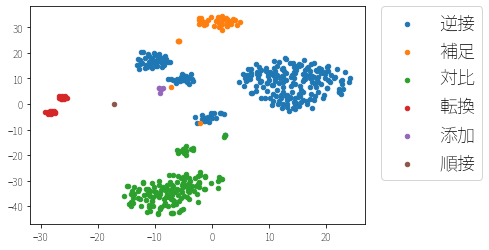
\includegraphics[width=80mm]{figure/tsne_true.png}
		\caption{正しい単語での t-SNE の結果}
		\label{tsne_true}
	\end{center}
  \begin{center}
    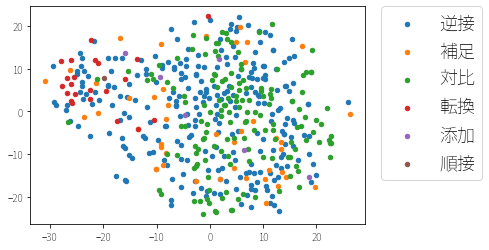
\includegraphics[width=80mm]{figure/tsne.png}
    \caption{[MASK] をかけたときの t-SNE の結果}
    \label{tsne}
  \end{center}
\end{figure}
単語数における精度の差について確認した.
図 \ref{tangosu1} に実験 1 において, 正解データ, 間違いデータそれぞれの全単語数の分布を示す.
なお, 正解数, 不正解数が合計で 1 になるようにそれぞれ正規化している.
\begin{figure}[ht]
	\begin{center}
		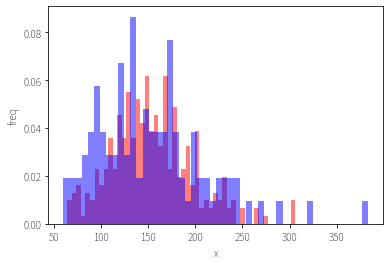
\includegraphics[width=80mm]{figure/tanosu_zikken1.png}
		\caption{単語数と精度の分布 実験 1}
		\label{tangosu1}
	\end{center}
\end{figure}
図 \ref{tangosu1}より, 正解データと間違いデータで分布の際は見られるものの, 特徴は顕著ではなかった.
このため, 文の長さは推定の精度に影響しないと考えられる. \par
次に, 語彙数について正解したものと間違えたもので比較した.
図 \ref{tangosyuruisu} に, 実験 1 において, 正解データ, 間違いデータそれぞれの
語彙数の分布を示す. どちらも正規化している.
\begin{figure}[ht]
	\begin{center}
		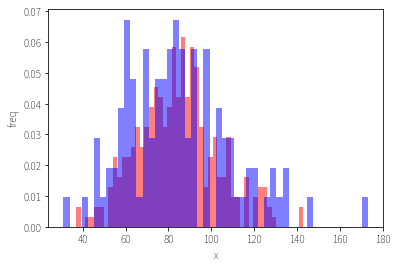
\includegraphics[width=80mm]{figure/goisu.png}
		\caption{語彙数と精度の分布 実験 1}
		\label{tangosyuruisu}
	\end{center}
\end{figure}
他の 2 つの実験でも同様の結果を示したので, 語彙数の分類精度への影響はほとんどないことが考えられる.
\section{まとめと今後の課題}
本稿では, 文章の 2 文間の接続詞が逆接かそうでないかの 2 クラスに分類し,
その分類精度を確認した.
結果, 接続詞の分散表現を得る手法の精度が最も高くなった.
また, 得られた結果を文間の接続詞ごとに分類することにより, 接続詞ごとに精度の差異が確認できた.
次に, 単語数や語彙数での精度の差を確認したところ, 単語数や語彙数による精度への影響を確認できなかった.
今後の課題として, 逆接以外の他の一つとそれ以外の分類, また, 多クラス分類をすることが挙げられる.
その際には, 種類ごとのデータ数の偏りを考慮したモデルにする必要がある.
また, 単語の各品詞ごとの精度の関係を確認することが挙げられる.
今後の展望として, 文間の接続詞の推定で高い精度の出るモデルを提案することがあげられる.
これにより文間に接続詞を含まない 2 文においても,
接続詞があると仮定した場合の接続詞を推定することで, 文同士の関係性の指標を得ることが可能になると考えられる.
その推定結果を既存の文章生成のパラメータに加えることで, 文同士の関係を考慮した文生成ができると予測される.
\bibliography{index}
\end{document}
